%!TEX root = ../main.tex

\chapter{总结和展望}

\section{相关工作总结}

本模板主要内容来源于ZJU-Awesome项目,
参考软件学院论文格式要求做出调整,
并加入补充宏包,调整若干属性配置完成。
封面方面主要调整了各栏间距和对齐,
摘要依照软件学院更改了关键字的样式和页码的样式。
软件学院规定从摘要起每页必须有对应章标题的页眉,
虽然在章头处排版页眉本不雅观,
但考虑到已经有以大部分同学使用Word字处理软件遵照执行,
为保一致性,本模板暂时向软件学院的设定妥协。
由于论文格式要求并未向章头处的间距做出任何设定,
本模板保留ZJU-Awesome设定。
除此之外,本模板还做出了不少微小的改动。
详情请仔细阅读\texttt{zjuthesis.cls}和\texttt{main.tex}相关内容。

考虑到大部分软件学院的同学对\LaTeX 论文排版的陌生,
本文以尽量精炼的篇幅介绍了论文排版工作的各方面。
现在给出一个参考流程如\autoref{fig:workflow} 希望能对初次使用
\LaTeX 排版论文的同学一点提示。

\begin{figure}[htbp]
    \centering
    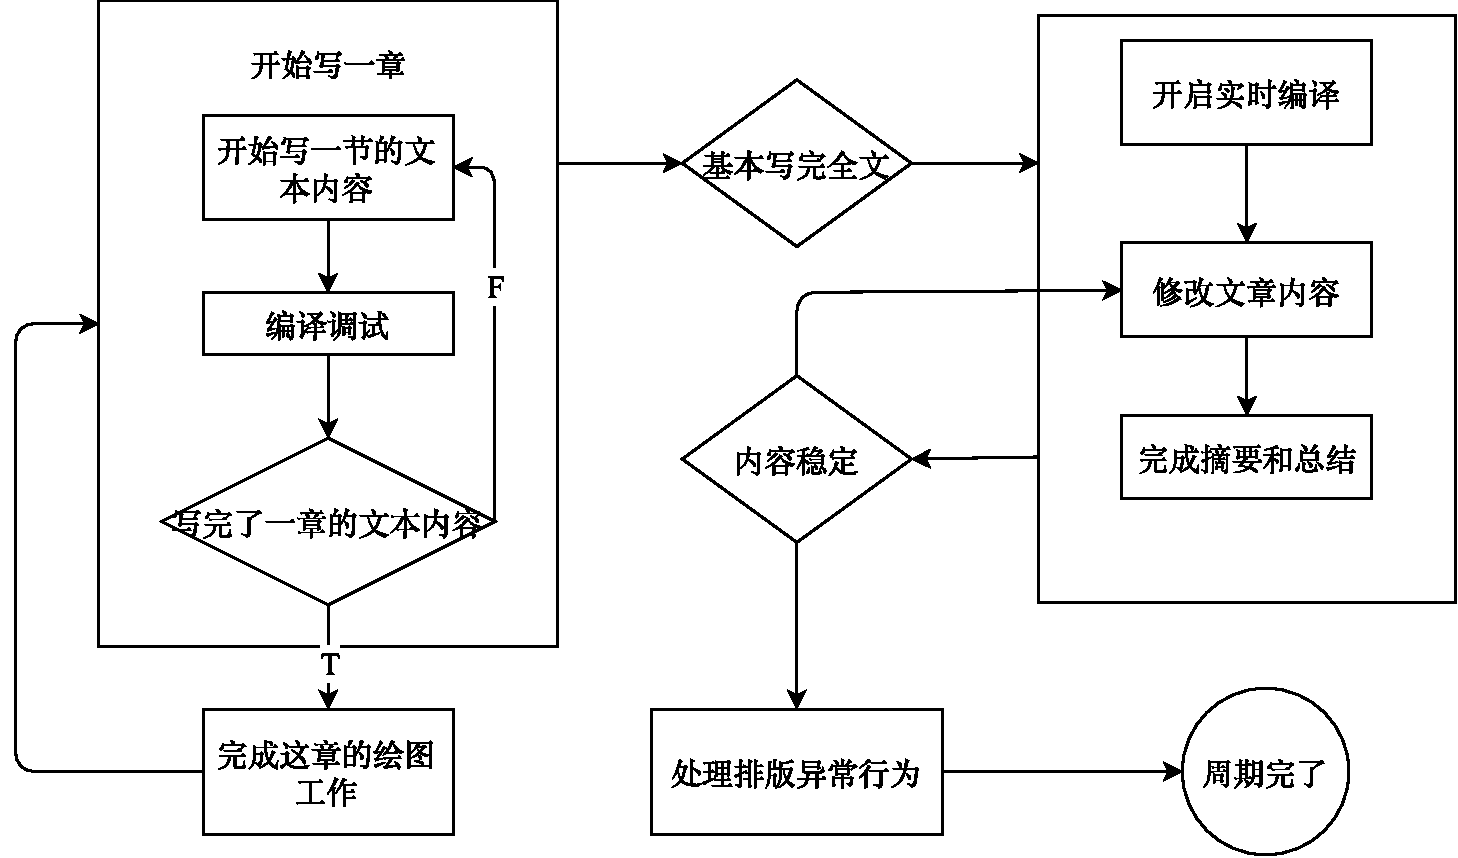
\includegraphics[width=.8\textwidth]{workflow.pdf}
    \caption{论文排版工作参考流程}
    \label{fig:workflow}
\end{figure}

\section{展望}

本文没有讨论各式\LaTeX 环境的使用细则,宏包的具体细节,
调试查错的技巧,也几乎没有交待任何一种具体的绘图方案。
本文希望屏幕前的你能以最少的时间代价完成论文排版工作,
养成到内容和样式完全分离的电子写作习惯,
并在对外输出知识时常思考最佳信息表达的模式。

本文草拟于2016年夏季毕业论文送审前,
希望本文能抛砖引玉。
对\LaTeX 有经验的后辈们若能继续完善甚至颠覆本模板的设定,
相信一定能对软件学院的论文排版素质起到根本的改善作用。

\section{真实参考资料}

考虑到下一页的参考文献是样例凑数,
此处不完整且不严谨地列出本文真实的参考资料:
\begin{description}
    \item[常规文档] \texttt{http://latexfly.com/docs/}
    \item[算法宏包] \texttt{https://en.wikibooks.org/wiki/LaTeX/Algorithms}
    \item[参考文献管理] \texttt{https://www.zhihu.com/question/23565739}
    \item[优雅的使用Word] \texttt{https://www.zhihu.com/question/20541531}
    \item[电子科大论文模板] \texttt{https://github.com/shifujun/UESTCthesis/wiki}
    \item[实时编译] \texttt{http://xiaoweiz.github.io/posts/2014/Aug/ST\_skim\_latexmk/}
    \item[一份不太简短的\LaTeX2e 介绍]   
    \item[各种宏包的手册] 在 TeX Live Utility 就可以查看
\end{description}
